%===============================================================================
% LaTeX sjabloon voor de bachelorproef toegepaste informatica aan HOGENT
% Meer info op https://github.com/HoGentTIN/latex-hogent-report
%===============================================================================

\documentclass[dutch,dit,thesis]{hogentreport}

% TODO:
% - If necessary, replace the option `dit`' with your own department!
%   Valid entries are dbo, dbt, dgz, dit, dlo, dog, dsa, soa
% - If you write your thesis in English (remark: only possible after getting
%   explicit approval!), remove the option "dutch," or replace with "english".

\usepackage{lipsum} % For blind text, can be removed after adding actual content

%% Pictures to include in the text can be put in the graphics/ folder
\graphicspath{{../graphics/}}

%% For source code highlighting, requires pygments to be installed
%% Compile with the -shell-escape flag!
%% \usepackage[chapter]{minted}
%% If you compile with the make_thesis.{bat,sh} script, use the following
%% import instead:s
\usepackage[chapter,outputdir=../output]{minted}
\usemintedstyle{solarized-light}
\usepackage{graphicx} % Voor het gebruik van \resizebox
\usepackage{placeins} % Voor strikt plaatsen van tabellen en figuren
\usepackage{float} % Voor H-plaatsing van figuren
\usepackage{hyperref} % Voor clickable links
\usepackage[version=4]{mhchem} % Voor chemische formules

%% Formatting for minted environments.
\setminted{%
    autogobble,
    frame=lines,
    breaklines,
    linenos,
    tabsize=4
}

%% Ensure the list of listings is in the table of contents
\renewcommand\listoflistingscaption{%
    \IfLanguageName{dutch}{Lijst van codefragmenten}{List of listings}
}
%%\renewcommand\listingscaption{%
    %%\IfLanguageName{dutch}{Codefragment}{Listing}
%%}
\renewcommand*\listoflistings{%
    \cleardoublepage\phantomsection\addcontentsline{toc}{chapter}{\listoflistingscaption}%
    \listof{listing}{\listoflistingscaption}%
}

% Other packages not already included can be imported here

%%---------- Document metadata -------------------------------------------------
% TODO: Replace this with your own information
\author{Wout Van Cleemput}
\supervisor{Karine Samyn}
\cosupervisor{Johan Decorte}
\title
    {Edge Computing voor \\ Real-time Omgevingsmonitoring: \\ Optimalisatie van \\  Datapartitionering in \\ Gedistribueerde Sensornetwerken}
\academicyear{\advance\year by -1 \the\year--\advance\year by 1 \the\year}
\examperiod{1}
\degreesought{\IfLanguageName{dutch}{Professionele bachelor in de toegepaste informatica}{Bachelor of applied computer science}}
\partialthesis{false} %% To display 'in partial fulfilment'
%\institution{Internshipcompany BVBA.}

%% Add global exceptions to the hyphenation here
\hyphenation{back-slash}

%% The bibliography (style and settings are  found in hogentthesis.cls)
\addbibresource{bachproef.bib}            %% Bibliography file
\addbibresource{../voorstel/voorstel.bib} %% Bibliography research proposal
\defbibheading{bibempty}{}

%% Prevent empty pages for right-handed chapter starts in twoside mode
\renewcommand{\cleardoublepage}{\clearpage}

\renewcommand{\arraystretch}{1.2}

%% Content starts here.
\begin{document}

%---------- Front matter -------------------------------------------------------

\frontmatter

\hypersetup{pageanchor=false} %% Disable page numbering references
%% Render a Dutch outer title page if the main language is English
\IfLanguageName{english}{%s
    %% If necessary, information can be changed here
    \degreesought{Professionele Bachelor toegepaste informatica}%
    \begin{otherlanguage}{dutch}%
       \maketitle%
    \end{otherlanguage}%
}{}

%% Generates title page content
\maketitle
\hypersetup{pageanchor=true}

%%=============================================================================
%% Voorwoord
%%=============================================================================

\chapter*{\IfLanguageName{dutch}{Woord vooraf}{Preface}}%
\label{ch:voorwoord}

%% TODO:
%% Het voorwoord is het enige deel van de bachelorproef waar je vanuit je
%% eigen standpunt (``ik-vorm'') mag schrijven. Je kan hier bv. motiveren
%% waarom jij het onderwerp wil bespreken.
%% Vergeet ook niet te bedanken wie je geholpen/gesteund/... heeft

Met veel enthousiasme presenteer ik mijn bachelorproef over de optimalisatie van gegevensopslag in Edge-omgevingen.

Dit onderwerp heeft mijn aandacht getrokken vanwege de opkomst van Edge computing en omdat ik mijn kennis over databases wou uitbreiden.

Het verkennen van Edge Database-architecturen biedt een fascinerende kijk op de evolutie van gegevensbeheer, en de impact die deze nieuwe technologieën hebben op de wereld van IT.

Ik wil graag mijn co-promotor, Kenneth Van den Berghe van het bedrijf optis en mijn begeleider Lieven Smits, bedanken voor hun begeleiding en feedback tijdens het schrijven van deze bachelorproef.

Ook wil ik mijn familie en vrienden bedanken voor hun steun en aanmoediging tijdens het schrijfproces.

Ik hoop dat deze bachelorproef een waardevolle bijdrage zal leveren aan het onderzoeksdomein en dat het lezers zal overtuigen om verder te gaan met dit interessante onderwerp.

%%=============================================================================
%% Samenvatting
%%=============================================================================

% TODO: De "abstract" of samenvatting is een kernachtige (~ 1 blz. voor een
% thesis) synthese van het document.
%
% Een goede abstract biedt een kernachtig antwoord op volgende vragen:
%
% 1. Waarover gaat de bachelorproef?
% 2. Waarom heb je er over geschreven?
% 3. Hoe heb je het onderzoek uitgevoerd?
% 4. Wat waren de resultaten? Wat blijkt uit je onderzoek?
% 5. Wat betekenen je resultaten? Wat is de relevantie voor het werkveld?
%
% Daarom bestaat een abstract uit volgende componenten:
%
% - inleiding + kaderen thema
% - probleemstelling
% - (centrale) onderzoeksvraag
% - onderzoeksdoelstelling
% - methodologie
% - resultaten (beperk tot de belangrijkste, relevant voor de onderzoeksvraag)
% - conclusies, aanbevelingen, beperkingen
%
% LET OP! Een samenvatting is GEEN voorwoord!

%%---------- Nederlandse samenvatting -----------------------------------------
%
% TODO: Als je je bachelorproef in het Engels schrijft, moet je eerst een
% Nederlandse samenvatting invoegen. Haal daarvoor onderstaande code uit
% commentaar.
% Wie zijn bachelorproef in het Nederlands schrijft, kan dit negeren, de inhoud
% wordt niet in het document ingevoegd.

\IfLanguageName{english}{%
\selectlanguage{dutch}
\chapter*{Samenvatting}
\lipsum[1-4]
\selectlanguage{english}
}{}

%%---------- Samenvatting -----------------------------------------------------
% De samenvatting in de hoofdtaal van het document

\chapter*{\IfLanguageName{dutch}{Samenvatting}{Abstract}}

\lipsum[1-4]


%---------- Inhoud, lijst figuren, ... -----------------------------------------

\tableofcontents

% In a list of figures, the complete caption will be included. To prevent this,
% ALWAYS add a short description in the caption!
%
%  \caption[short description]{elaborate description}
%
% If you do, only the short description will be used in the list of figures

\listoffigures

% If you included tables and/or source code listings, uncomment the appropriate
% lines.
\listoftables

\listoflistings

% Als je een lijst van afkortingen of termen wil toevoegen, dan hoort die
% hier thuis. Gebruik bijvoorbeeld de ``glossaries'' package.
% https://www.overleaf.com/learn/latex/Glossaries

%---------- Kern ---------------------------------------------------------------

\mainmatter{}

% De eerste hoofdstukken van een bachelorproef zijn meestal een inleiding op
% het onderwerp, literatuurstudie en verantwoording methodologie.
% Aarzel niet om een meer beschrijvende titel aan deze hoofdstukken te geven of
% om bijvoorbeeld de inleiding en/of stand van zaken over meerdere hoofdstukken
% te verspreiden!

%%=============================================================================
%% Inleiding
%%=============================================================================

\chapter{\IfLanguageName{dutch}{Inleiding}{Introduction}}%
\label{ch:inleiding}

In deze inleiding geef ik een overzicht van het onderwerp van mijn bachelorproef, waarin ik de impact van data-partitioneringstechnieken op de prestaties van databases.
Het doel is om te evalueren hoe deze technieken kunnen worden ingezet in een eenvoudige en praktische Edge Computing-context die relevant is voor Optis, een consultancybedrijf gespecialiseerd in IT-oplossingen. Als concrete use case wordt het optimaliseren van data-opslag en verwerking in een IoT-omgeving onderzocht, waarbij uitdagingen zoals hoge latentie en inefficiënt bandbreedtegebruik aangepakt worden.

\section{\IfLanguageName{dutch}{Probleemstelling}{Problem Statement}}%
\label{sec:probleemstelling}

De kernprobleemstelling van deze studie is het verbeteren van de efficiëntie van gegevensopslag en -verwerking in een IoT-omgeving. 
Optis ondersteunt klanten bij het implementeren van IT-oplossingen in gedistribueerde systemen. Veel van deze klanten werken met IoT-apparaten zoals sensoren en monitoringtools. Deze apparaten genereren grote hoeveelheden gegevens die moeten worden opgeslagen en verwerkt. 
Dit leidt vaak tot problemen zoals lange responstijden, inefficiënte data-overdracht en schaalbaarheidsbeperkingen. Deze uitdagingen vereisen oplossingen die gericht zijn op lokaal databeheer, ondersteund door effectieve data-partitioneringstechnieken.

\section{\IfLanguageName{dutch}{Onderzoeksvraag}{Research question}}%
\label{sec:onderzoeksvraag}

De centrale onderzoeksvraag die in deze studie wordt behandeld, is: 
\\ "Hoe beïnvloeden data-partitioneringstechnieken in combinatie met edge-databases de prestaties \\ van een Edge Computing omgeving van Optis?" \\ 
  Deze vraag richt zich op hoe data-partitioneringstechnieken de prestaties van edge-databases beïnvloeden binnen een Edge Computing-omgeving. Het doel van het onderzoek is om zowel de prestaties van databases te verbeteren als een geschikte edge-database te identificeren voor gebruik in deze context.

\section{\IfLanguageName{dutch}{Onderzoeksdoelstelling}{Research objective}}%
\label{sec:onderzoeksdoelstelling}

Het doel van dit onderzoek is om praktische aanbevelingen te formuleren voor Optis door de impact van verschillende data-partitioneringstechnieken op de prestaties van databases te analyseren binnen een eenvoudige simulatie. Deze studie zal bijdragen aan het begrijpen van de toepasbaarheid van partitioneringstechnieken in een kleine, schaalbare context en zal praktische inzichten bieden die door Optis verder kunnen worden toegepast.

\begin{itemize}
  \item Het uitvoeren van een gedetailleerde evaluatie van de impact van data-partitioneringstechnieken op de prestaties van edge-databases in een IoT-omgeving.
  \item Het ontwikkelen van een proof of concept om te onderzoeken hoe deze technieken de latentie, bandbreedte en schaalbaarheid beïnvloeden in een Edge Computing-context.
  \item Het formuleren van praktische aanbevelingen voor Optis op basis van de resultaten van de proof of concept.
\end{itemize}

\section{\IfLanguageName{dutch}{Opzet van deze bachelorproef}{Structure of this bachelor thesis}}%
\label{sec:opzet-bachelorproef}

De rest van deze bachelorproef is als volgt opgebouwd:

In Hoofdstuk 2 wordt een overzicht gegeven van de stand van zaken binnen het onderzoeksdomein door middel van een literatuurstudie. Deze studie richt zich op de mogelijkheden en uitdagingen van Edge Computing, relevante data-partitioneringstechnieken, en de prestaties van bestaande Edge-databases.

In Hoofdstuk 3 wordt de methodologie besproken. Hier worden de gekozen onderzoeksmethoden en gebruikte technieken toegelicht, waaronder de proof of concept om de impact van data-partitioneringstechnieken te evalueren.

In Hoofdstuk 4 worden de resultaten gepresenteerd en geanalyseerd, waarbij een antwoord wordt geformuleerd op de onderzoeksvraag en aanbevelingen voor toekomstig onderzoek in dit domein worden besproken.

\section{\IfLanguageName{dutch}{Deelvragen}{Sub-questions}}%
\label{sec:deelvragen}

Om de onderzoeksvraag verder te verduidelijken en te structureren, worden de volgende deelvragen behandeld:
\begin{itemize}
    \item Hoe verhouden verschillende data-partitioneringstechnieken zich in termen van latentie in een Edge-omgeving?
    \item Wat is de invloed van data-partitioneringstechnieken op bandbreedteverbruik en netwerkprestaties in gedistribueerde Edge-netwerken?
    \item Hoe beïnvloeden deze technieken de schaalbaarheid van databases in een dynamische Edge-omgeving?
    \item Welke bestaande Edge-databasetechnologieën leveren, gemeten aan de hand van latentie, fouttolerantie en schaalbaarheid, de beste prestaties in combinatie met de onderzochte partitioneringstechnieken binnen de context van Optis?
\end{itemize}

\chapter{\IfLanguageName{dutch}{Stand van zaken}{State of the art}}%
\label{ch:stand-van-zaken}

Dit hoofdstuk biedt een uitgebreide literatuurstudie over EdgeDB als een tijdreeksdatabase voor het beheren van grote hoeveelheden tijdreeksgegevens, als onderdeel van deze bachelorproef.

Het is bedoeld om een grondige analyse te geven van de huidige stand van zaken binnen het onderzoeksdomein.

De inhoud van dit hoofdstuk bouwt voort op de inleiding en heeft als doel de lezer volledig op de hoogte te brengen van recente ontwikkelingen, technologieën en benaderingen die relevant zijn voor dit onderwerp, zodat zij het verdere verloop van de bachelorproef kunnen begrijpen zonder verdere opzoekingen te moeten doen.

\section{Bronnen zoekmethode}
De bronnen voor deze literatuurstudie werden gevonden door middel van een systematische zoekmethode, waarbij gebruik werd gemaakt van verschillende zoekmachines en databases, waaronder Google Scholar, IEEE Xplore, Semanthic Scolar en Elicit.
Als zoektermen gebruikten we "EdgeDB", "Database on Edge" en "Edge Computing".

\section{Database on Edge}

Database on Edge is een opkomende benadering binnen database technologie, voortkomend uit het gebruik van Edge computing \autocite{Yang2019EdgeDBAE}.

In tegenstelling tot traditionele databases worden Edge databases verspreid over verschillende lokale apparaten, waardoor gegevens lokaal verwerkt en opgeslagen kunnen worden, in plaats van centraal in de cloud.

Deze innovatieve benadering richt zich, vergelijkbaar met moderne bedrijven die streven naar efficiëntie en innovatie, op het verminderen van latency en het verbeteren van de prestaties.

Het concept is ontstaan uit de noodzaak om real-time interacties mogelijk te maken, wat cruciaal is in diverse toepassingen \autocite{Yang2019EdgeDBAE}.

Voordelen van Database on Edge omvatten lokale gegevensverwerking, verminderde latency en verbeterde prestaties, waardoor het geschikt is voor toepassingen waar snelle respons cruciaal is.

Echter, zoals bij elke technologische benadering, zijn er uitdagingen verbonden aan Database on Edge, waaronder het beheer van diverse databases over verschillende apparaten, optimalisatie van resourcegebruik op Edge Devices, en het waarborgen van consistente prestaties.

De optimalisatie van Database on Edge is een actief onderzoeksgebied en omvat het verkennen van efficiënte algoritmen voor gegevensverwerking, verbeteringen in gegevensopslag, en het beheer van gedistribueerde databases om de prestaties te maximaliseren.

\section{Tijdreeksdatabases}

Tijdreeksdatabases zijn van essentieel belang in moderne informatiesystemen, met toepassingen variërend van IoT (Internet of Things) tot financiële analyses en meer.

Dit gespecialiseerde type database is geoptimaliseerd voor het opslaan, beheren en analyseren van tijdreeksgegevens, waarbij elk gegevenspunt wordt geassocieerd met een tijdstempel. 

In de afgelopen jaren zijn verschillende tijdreeksdatabases ontwikkeld om te voldoen aan de specifieke behoeften van verschillende toepassingsgebieden.

Voorbeelden hiervan zijn BTrDB en InfluxDB, twee bekende tijdreeksdatabases die elk hun eigen benaderingen en optimalisaties bieden voor het verwerken van tijdreeksgegevens \autocite{Yang2019EdgeDBAE}.

\section{EdgeDB: Een nieuwe benadering voor tijdreeksdatabases}

EdgeDB is een recente toevoeging aan het landschap van tijdreeksdatabases en belooft een innovatieve benadering te bieden voor het beheren van tijdreeksgegevens.

Deze nieuwe database introduceert nieuwe indexstructuren en queryverwerkingstechnieken om de prestaties en efficiëntie te verbeteren.

Een van de belangrijkste kenmerken van EdgeDB is het gebruik van TMTree, een geoptimaliseerde indexstructuur die is ontworpen om schrijfoperaties te optimaliseren en het geheugengebruik te minimaliseren \autocite{Yang2019EdgeDBAE}.

\section{Vergelijkende evaluatie van EdgeDB}

Een grondige evaluatie van EdgeDB is essentieel om de prestaties en bruikbaarheid van deze nieuwe tijdreeksdatabase te begrijpen in vergelijking met bestaande oplossingen zoals BTrDB en InfluxDB.

Verschillende evaluatiemetrics worden gebruikt, waaronder insert-prestaties, schrijfprestaties, query-prestaties, geheugenoverhead en invoersnelheid van TMTree.

Deze evaluatie biedt inzicht in de sterke punten en beperkingen van EdgeDB en helpt bij het bepalen van de geschiktheid ervan voor verschillende toepassingsgebieden en gebruiksscenario's \autocite{Yang2019EdgeDBAE}.

\section{VergeDB: Een innovatieve tijdreeksdatabase voor Edge Computing}

Een recente ontwikkeling op het gebied van tijdreeksdatabases is VergeDB, een database die specifiek is ontworpen voor IoT-analytics op Edge-apparaten \autocite{Paparrizos2021VergeDBAD}. VergeDB belooft een innovatieve benadering te bieden voor het beheren van tijdreeksgegevens op de rand van het netwerk, wat cruciaal is voor real-time toepassingen waarbij snelle respons vereist is.

Deze nieuwe database introduceert nieuwe compressiemethoden, indexstructuren en queryverwerkingstechnieken om de prestaties en efficiëntie te verbeteren. Een van de belangrijkste kenmerken van VergeDB is de mogelijkheid om gegevens lokaal op te slaan en te verwerken op Edge-apparaten, waardoor de latentie wordt verminderd en de prestaties worden verbeterd.

VergeDB biedt ook ondersteuning voor geavanceerde analysetaken en machine learning-taken, zoals trendanalyse, patroonherkenning en anomaliedetectie, waardoor het een veelzijdige oplossing is voor diverse toepassingen op het gebied van IoT-analytics.

Deze nieuwe benadering van tijdreeksdatabases op de rand van het netwerk opent nieuwe mogelijkheden voor het efficiënt beheren en analyseren van tijdreeksgegevens in real-time, wat essentieel is voor het succes van IoT-toepassingen in verschillende domeinen.

\section{Conclusie}
Database on Edge, voortkomend uit het gebruik van Edge computing, biedt veelbelovende voordelen zoals lokale gegevensverwerking, verminderde latency en verbeterde prestaties. Echter, er zijn ook uitdagingen verbonden aan deze benadering, zoals het beheer van diverse databases over verschillende apparaten en het optimaliseren van resourcegebruik op Edge Devices.

EdgeDB en VergeDB vertegenwoordigen nieuwe benaderingen voor het beheren van tijdreeksgegevens op de rand van het netwerk, met innovatieve functies zoals geoptimaliseerde indexstructuren en queryverwerkingstechnieken. Deze benaderingen openen nieuwe mogelijkheden voor het efficiënt beheren en analyseren van tijdreeksgegevens in real-time, wat essentieel is voor het succes van IoT-toepassingen in verschillende domeinen.

De volgende stap in dit onderzoek is de methodologie voor de vergelijkende evaluatie van EdgeDB te beschrijveb. Dit zal helpen bij het beoordelen van de prestaties en bruikbaarheid van EdgeDB in vergelijking met andere tijdreeksdatabases, en zal verdere inzichten bieden in de geschiktheid ervan voor verschillende toepassingsgebieden en gebruiksscenario's.

%%=============================================================================
%% Methodologie
%%=============================================================================

\chapter{\IfLanguageName{dutch}{Methodologie}{Methodology}}%
\label{ch:methodologie}

%% TODO: In dit hoofstuk geef je een korte toelichting over hoe je te werk bent
%% gegaan. Verdeel je onderzoek in grote fasen, en licht in elke fase toe wat
%% de doelstelling was, welke deliverables daar uit gekomen zijn, en welke
%% onderzoeksmethoden je daarbij toegepast hebt. Verantwoord waarom je
%% op deze manier te werk gegaan bent.
%% 
%% Voorbeelden van zulke fasen zijn: literatuurstudie, opstellen van een
%% requirements-analyse, opstellen long-list (bij vergelijkende studie),
%% selectie van geschikte tools (bij vergelijkende studie, "short-list"),
%% opzetten testopstelling/PoC, uitvoeren testen en verzamelen
%% van resultaten, analyse van resultaten, ...
%%
%% !!!!! LET OP !!!!!
%%
%% Het is uitdrukkelijk NIET de bedoeling dat je het grootste deel van de corpus
%% van je bachelorproef in dit hoofstuk verwerkt! Dit hoofdstuk is eerder een
%% kort overzicht van je plan van aanpak.
%%
%% Maak voor elke fase (behalve het literatuuronderzoek) een NIEUW HOOFDSTUK aan
%% en geef het een gepaste titel.

In dit hoofdstuk wordt de aanpak van het onderzoek toegelicht. 
 Om de onderzoeksvraag te beantwoorden wordt een combinatie van literatuurstudie, een vergelijkende analyse en een proof of concept toegepast.

De proof of concept richt zich op het implementeren en testen van databases die gebruikmaken van verschillende partitioneringstechnieken.
 De prestaties van deze databases worden gemeten op basis van gedefinieerde criteria zoals snelheid, schaalbaarheid en betrouwbaarheid in een Edge-omgeving.

De technische diepte van deze bachelorproef wordt benadrukt,
 inclusief de beschrijving van gebruikte tools zoals hardware, software en diensten. \\

Een gedetailleerde tijdsplanning wordt opgesteld om de duur van elke onderzoeksfase en de concrete deliverables te definiëren.
Deze tijdsplanning wordt opgesteld in de vorm van een Gantt chart en een flowchart. Deze zal u vinden op de laatste pagina van dit voorstel.

Het onderzoek verloopt in vier fases, die elk gericht zijn op bepaalde doelstellingen en methoden. \\

\section*{Fase 1: Literatuurstudie}

\textbf{Doelstelling:}  
Inzicht krijgen in data-partitioneringstechnieken, vereisten van edge-databases en toepassingen in sensornetwerken.

\textbf{Aanpak:}
\begin{itemize}
    \item Analyse van wetenschappelijke literatuur en officiële documentatie.
    \item Identificatie van functionele en niet-functionele vereisten voor databases in edge-omgevingen.
    \item Opstellen van een longlist van mogelijke databases en technieken.
\end{itemize}

\textbf{Beantwoorde deelvragen:}
\begin{itemize}
    \item \textbf{Welke uitdagingen ontstaan bij het verwerken van grote hoeveelheden IoT-data in een centrale cloudomgeving?} \\ 
    Literatuur toont aan waar cloudverwerking tekortschiet in netwerken met veel sensoren.
    \item \textbf{Wat zijn de functionele vereisten van databases voor het verwerken van real-time sensordata in een edge-context met beperkte connectiviteit?} \\
    Deze vraag wordt beantwoord aan de hand van een literatuurstudie naar bestaande databaseoplossingen die geschikt zijn voor gebruik in edge-omgevingen met sensornetwerken.
\end{itemize}

\textbf{Deliverable:} Een overzicht van de belangrijkste inzichten omtrent partitionering, edge computing en real-time monitoring. \\
\textbf{Deadline:} 21/11/2024

\section*{Fase 2: Selectie en vergelijking van databases}

\textbf{Doelstelling:}  
Databasetechnologieën identificeren die geschikt zijn voor edge-omgevingen en deze theoretisch vergelijken op basis van relevante criteria.

\textbf{Aanpak:}
\begin{itemize}
    \item Opstellen van evaluatiecriteria zoals latentie, fouttolerantie, schaalbaarheid en gebruiksgemak.
    \item Selectie van drie geschikte databases: Cassandra, MongoDB en TimescaleDB.
    \item Vergelijkende analyse van deze databases aan de hand van documentatie en bestaande benchmarks.
\end{itemize}

\textbf{Beantwoorde deelvraag:}
\begin{itemize}
    \item \textbf{Welke van de geselecteerde edge-databases leveren de beste prestaties op vlak van latentie, fouttolerantie en schaalbaarheid binnen de HoGent-use case?} \\
    De vergelijkende studie onderzoekt de prestaties van de databases en hun mogelijke geschiktheid voor de use case.
\end{itemize}

\textbf{Deliverable:} Een gemotiveerde shortlist met drie geschikte edge-databases. \\
\textbf{Deadline:} 05/12/2024

\section*{Fase 3: Proof of Concept}

\textbf{Doelstelling:}  
De geselecteerde databases implementeren in een gesimuleerde edge-omgeving en hun prestaties testen met voorbeeldgegevens.

\textbf{Aanpak:}
\begin{itemize}
    \item Opzetten van een testomgeving met Docker Compose die een edge-scenario nabootst.
    \item Genereren van testdata die sensorwaardes simuleert (CO₂, druk, temperatuur om de 5 seconden).
    \item Implementeren van list-based en range-based partitionering.
    \item Testen op latency, schaalbaarheid, foutafhandeling en beschikbaarheid.
    \item Verzamelen en analyseren van meetgegevens via scripts.
\end{itemize}

\textbf{Beantwoorde deelvragen:}
\begin{itemize}
    \item \textbf{Hoe beïnvloeden verschillende data-partitioneringstechnieken de latentie bij dataverwerking in een Edge Computing-omgeving?} \\
    Door latency te meten in verschillende opstellingen met verschillende technieken.
    \item \textbf{Wat is het effect van verschillende data-partitioneringstechnieken op de netwerkbelasting bij het verwerken van real-time sensordata in een gedistribueerd sensornetwerk?} \\
    Netwerkverkeer wordt gemeten tijdens het testen van de technieken.
    \item \textbf{Wat is de impact van partitioneringsstrategieën op de schaalbaarheid van edge-databases bij toenemende datavolumes?} \\
    Door het effect van groeiende datasets te analyseren bij elke techniek.
\end{itemize}

\textbf{Deliverable:} Een rapport met testresultaten, grafieken en evaluatie per techniek en database. \\
\textbf{Deadline:} 24/12/2024

\section*{Fase 4: Analyse en evaluatie}

\textbf{Doelstelling:}  
Conclusies trekken over welke database en partitioneringstechniek de beste prestaties leveren in deze edge-context.

\textbf{Aanpak:}
\begin{itemize}
    \item Analyse van testresultaten uit de PoC.
    \item Vergelijking op basis van prestatiecriteria.
    \item Formuleren van aanbevelingen voor toekomstige toepassingen.
    \item Bepalen van een totaalscore per database aan de hand van genormaliseerde prestatie-indicatoren, waarbij elke indicator gewogen wordt op basis van de relevantie voor edge computing.
\end{itemize}

\textbf{Beantwoorde deelvraag:}
\begin{itemize}
    \item \textbf{Welke van de geselecteerde edge-databases leveren de beste prestaties op vlak van latentie, fouttolerantie en schaalbaarheid binnen de HoGent-use case?} \\
    De analyse van de testresultaten toont welke oplossing het best past bij de gesimuleerde toepassing.
\end{itemize}

\textbf{Deliverable:} Een eindrapport met visuele samenvattingen, conclusies en aanbevelingen. Inclusief een rangschikking van alle databases op basis van genormaliseerde prestatiecriteria en bijbehorende wegingsfactoren. \\
\textbf{Deadline:} 05/01/2025

% Voeg hier je eigen hoofdstukken toe die de ``corpus'' van je bachelorproef
% vormen. De structuur en titels hangen af van je eigen onderzoek. Je kan bv.
% elke fase in je onderzoek in een apart hoofdstuk bespreken.

%\input{...}
%\input{...}
%...

\chapter{\IfLanguageName{dutch}{Proof of concept}{Proof of concept}}%
\label{ch:proof-of-concept}

\section{Proof of Concept: Real-time Monitoring via Centrale en Edge Databases}

Deze proof of concept heeft als doel het prestatieverschil te analyseren tussen twee implementaties voor real-time monitoring: een traditionele centrale database-architectuur (Gebouw A) en een edge computing-architectuur met lokale verwerking (Gebouw B). De focus ligt op typische IoT-sensordata zoals \ce{CO2}-metingen, temperatuur en luchtdruk.

Beide scenario's worden opgezet met Docker Compose om gescheiden en reproduceerbare testomgevingen te garanderen. Binnen elk scenario worden verschillende databases getest met meerdere datapartitioneringstechnieken (zoals range-based en list-based partitionering) om te bepalen welke het meest geschikt is voor centrale versus gedistribueerde verwerking.
\section{Functionele en niet-functionele Eisen}

\subsection{Functionele eisen}

De functionele eisen beschrijven wat het systeem concreet moet doen. Voor deze proof of concept binnen de HoGent-use case werden volgende functionele eisen gedefinieerd:

\begin{itemize}
    \item Het systeem moet om de 5 seconden de waarden van \ce{CO2}, temperatuur en luchtdruk registreren.
    \item Het systeem moet een waarschuwing tonen wanneer de \ce{CO2}-waarde de drempel van 800 ppm overschrijdt.
    \item Het systeem moet real-time grafieken tonen met de evolutie van de \ce{CO2}-waarden.
    \item Het systeem moet historische meetgegevens kunnen opvragen per lokaal.
    \item Het systeem moet logs bijhouden van wanneer drempelwaarden zijn overschreden.
    \item Het systeem moet foutmeldingen tonen bij verbindingsproblemen met de database of edge-node.
\end{itemize}

\subsection{Niet-functionele eisen}

Niet-functionele eisen beschrijven de kwaliteitseigenschappen van het systeem. Dit zijn de niet-functionele eisen voor het systeem:

\begin{itemize}
    \item \textbf{Performantie (Must):} Het systeem moet lage latentie hebben ($<$ 500 ms) bij het tonen van nieuwe meetdata.
    \item \textbf{Schaalbaarheid (Must):} Het systeem moet uitbreidbaar zijn naar meerdere lokalen zonder herconfiguratie. Ook horizontale schaalbaarheid over meerdere nodes moet ondersteund worden zonder prestatiedaling.
    \item \textbf{Fouttolerantie (Must):} Het systeem moet blijven functioneren bij netwerkstoringen of node-uitval, zonder dataverlies.
    \item \textbf{Offline werking en synchronisatie (Should):} Het systeem moet tijdelijk lokaal data kunnen opslaan en veilig synchroniseren zodra netwerkverbinding is hersteld.
    \item \textbf{Lokale verwerking (Must):} De edge-node moet in staat zijn om data lokaal te verwerken om latentie en netwerkbelasting te minimaliseren.
    \item \textbf{Geheugengebruik en CPU-belasting (Should):} De database moet efficiënt werken op edge-devices met beperkte hardwarecapaciteit.
    \item \textbf{Doorvoersnelheid (Must):} Het systeem moet hoge frequenties van sensordata kunnen verwerken (inserts per seconde).
    \item \textbf{Gegevensconsistentie (Must):} Alle nodes moeten beschikken over een betrouwbare en gelijke data.
    \item \textbf{Beheer en onderhoud (Should):} De configuratie, monitoring en foutafhandeling van het systeem moeten eenvoudig zijn.
    \item \textbf{Beveiliging (Must):} Data moet veilig worden opgeslagen en enkel toegankelijk zijn voor bevoegde gebruikers.
    \item \textbf{Automatische compressie en retentie (Could):} Het systeem moet automatisch oudere gegevens kunnen comprimeren of verwijderen. Zo blijft de opslag beperkt en raakt de edge-node niet vol. Bijvoorbeeld: alleen de data van de laatste 7 dagen wordt volledig bewaard, oudere data wordt samengevat of verwijderd.
\end{itemize}

\section{Architectuur van de testopstelling}
\label{sec:architectuur-testopstelling}

De testopstelling is gebaseerd op een simulatie van een school met twee gebouwen: Gebouw A en Gebouw B. Elk gebouw stelt een ander soort database-architectuur voor. Op die manier kan getest worden wat het verschil is tussen centrale opslag van data en lokale verwerking aan de rand van het netwerk (edge computing).

\subsection{Gebouw A: Centrale verwerking}

Gebouw A stelt een centrale serverruimte voor waar alle meetgegevens verzameld worden. De data van de sensoren wordt naar deze centrale locatie gestuurd. Daar worden de gegevens opgeslagen en verwerkt met behulp van de databases MongoDB, Cassandra of TimescaleDB. Alles gebeurt dus op een centrale plaats, zonder verdeling over meerdere locaties.

\subsection{Gebouw B: Edge-verwerking per lokaal}

Gebouw B stelt een edge-omgeving voor. In dit gebouw heeft elk lokaal zijn eigen edge-node, dus zijn eigen kleine database. In totaal zijn er zes lokalen (B101 tot B106). Elk lokaal gebruikt een andere combinatie van database en partitionering:

\begin{itemize}
  \item B101: MongoDB met list-partitionering
  \item B102: MongoDB met range-partitionering
  \item B103: Cassandra met list-partitionering
  \item B104: Cassandra met range-partitionering
  \item B105: TimescaleDB met list-achtige partitionering
  \item B106: TimescaleDB met range-partitionering
\end{itemize}

De sensordata wordt lokaal opgeslagen en verwerkt. Als bijvoorbeeld het \ce{CO2}-niveau te hoog is, wordt dit direct opgemerkt door de lokale database, zonder dat de centrale server daarvoor nodig is. De edge-databases communiceren niet met elkaar en ook niet met Gebouw A. Zo kunnen de prestaties van elk systeem apart worden gemeten.

\subsection{Verschil in resources tussen centrale en edge-opstelling}

Om het verschil tussen een centrale en een edge-architectuur realistisch te simuleren, werden in Docker Compose verschillende CPU en geheugenlimieten ingesteld.
 De centrale node (Gebouw A) krijgt meer resources, terwijl de edge-nodes (Gebouw B) beperkter geconfigureerd zijn.
Op die manier wordt het verschil gesimuleerd tussen een datacenteromgeving en een edge-device zoals een Raspberry Pi of IoT-controller.
 Dit benadert de typische situatie waarbij centrale systemen op krachtige infrastructuur draaien en edge-devices gebruikmaken van beperkte hardware.
\begin{table}[H]
\centering
\begin{resizebox}{\textwidth}{!}{
  \begin{tabular}{|l|c|c|}
  \hline
  \textbf{Eigenschap} & \textbf{Centrale databases (Gebouw A)} & \textbf{Edge-databases (Gebouw B)} \\
  \hline
  Geheugen (RAM) & 1024MB (1 GB) & 512MB of 768MB \\
  CPU-limiet & 1.0 core & 1.0 core \\
  Verbinding & Permanent (stabiel netwerk) & Mogelijk onstabiel of tijdelijk offline \\
  Voorbeelden van containers & \texttt{timescaledb-central}, \texttt{mongodb-central} & \texttt{mongos2}, \texttt{cassandra-edge-range}, \texttt{timescaledb-edge-list} \\
  \hline
  \end{tabular}
}
\end{resizebox}
\caption{Simulatie van resourceverschillen tussen centrale en edge-opstellingen.}
\label{tab:resources}
\end{table}

\subsection{Visueel overzicht van de architectuur}

De onderstaande figuur toont hoe de opstelling eruitziet. Links staat Gebouw A met de drie centrale databases. Rechts staan de zes lokalen van Gebouw B, elk met hun eigen edge-database. Er is geen verbinding tussen de gebouwen tijdens de tests, zodat de resultaten per systeem goed vergeleken kunnen worden.

\begin{figure}[H]
  \centering
  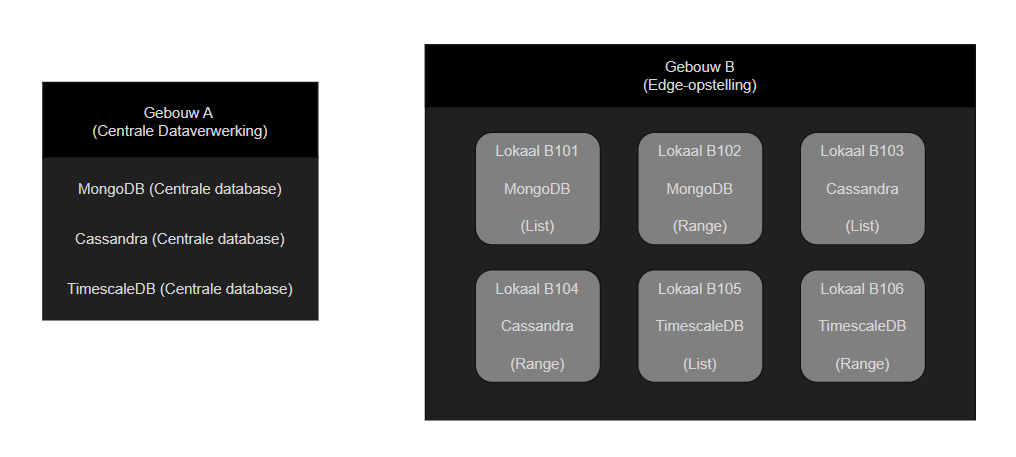
\includegraphics[width=\textwidth]{SchemaPoC.png}
  \caption{Overzicht van de testopstelling. Elke ruimte in Gebouw B heeft een eigen edge-database. In Gebouw A worden de centrale databases getest.}
  \label{fig:school-architectuur}
\end{figure}

\subsection{Testdoelen in beide gebouwen:}
\begin{itemize}
    \item Verzamelen en opslaan van meetgegevens vanuit meerdere lokalen.
    \item Detectie van drempelwaarden (\ce{CO2} > 800 ppm) en genereren van waarschuwingen.
    \item Logging van drempeloverschrijdingen en opvraging van historische data.
    \item Evaluatie van systeemprestaties bij verhoogde belasting.
    \item Analyse van schaalbaarheid en gedrag bij uitbreiding naar meerdere lokalen.
    \item Meting van latency en doorvoersnelheid.
    \item Fouttolerantie en gedrag bij netwerkstoringen of node-uitval.
    \item Monitoring van resourcegebruik (CPU, geheugen).
\end{itemize}

\section{Ontwikkeling van de Applicatie}

De proof of concept is gerealiseerd met Docker Compose en gesimuleerde sensordata. De werking van de applicatie wordt getest aan de hand van concrete functionele eisen zoals het genereren van een waarschuwing wanneer het \ce{CO2}-gehalte hoger is dan 800 ppm.
Cassandra werd in deze proof of concept via Docker gebruikt op een virtuele edge-server per lokaal. Hoewel dit geen echte IoT-hardware is, vormt het een goede benadering om de prestaties en partitionering van Cassandra in een edge-omgeving te testen.

\subsection{Architectuur}

De applicatie is opgebouwd als een real-time monitoringdashboard in een edge-omgeving met volgende componenten:

\begin{itemize}
    \item \textbf{IoT-sensor (gesimuleerd):} Genereert elke 5 seconden meetgegevens.
    \item \textbf{Edge-node:} Verwerkt en slaat lokaal data op met een te testen database-engine.
    \item \textbf{Backend (ASP.NET Core):} Verwerkt sensordata, detecteert overschrijding van drempelwaarden en verstuurt meldingen.
    \item \textbf{Frontend (React):} Visualiseert live-data en historische grafieken.
    \item \textbf{Docker Compose:} Beheert de opstelling van verschillende databases, backend en frontend in afzonderlijke containers.
\end{itemize}

\subsection{Melding bij \ce{CO2}-overschrijding}

Bij overschrijding van 800 ppm \ce{CO2}:
\begin{itemize}
    \item Wordt een rode waarschuwing getoond op het dashboard.
    \item Wordt een log-item toegevoegd aan de database.
    %\item (Optioneel) Wordt een melding verstuurd via e-mail of webhook.
\end{itemize}

\section{Tabellen en Datastructuren}

De gebruikte tabel heet \texttt{sensor\_data} en heeft een consistente structuur in alle databases.

\paragraph{Velden in \texttt{sensor\_data}:}
\begin{itemize}
    \item \texttt{sensor\_id (UUID)} - Unieke identificatie per sensor.
    \item \texttt{timestamp (TIMESTAMP)} - Tijdstip van de meting.
    \item \texttt{temperature (DOUBLE)} - Temperatuurwaarde.
    \item \texttt{co2 (INTEGER)} - CO₂-waarde in ppm.
    \item \texttt{pressure (DOUBLE)} - Luchtdruk in hPa.
    \item \texttt{status (TEXT)} - Sensorstatus ('actief', 'offline').
\end{itemize}

\paragraph{Toepassing per architectuur:}
\begin{itemize}
    \item \textbf{Gebouw A (centraal):} verschillende databases worden getest als centrale opslagoptie voor data uit alle lokalen.

    \item \textbf{Gebouw B (edge):} elk lokaal heeft een eigen edge-node waarop verschillende edge-geschikte databases worden getest.
\end{itemize}

\subsection{Uitgevoerde queries per database}
Tijdens de tests werden de sensordata telkens via een specifieke query ingevoegd in de databanken. 
De queries verschillen per database-engine en partitioneringsstrategie. Hieronder worden de belangrijkste voorbeelden weergegeven.

\paragraph{Cassandra (centraal):}
\begin{verbatim}
INSERT INTO sensor_data (id, timestamp, temperature, co2, pressure, building, room)
VALUES (?, ?, ?, ?, ?, ?, ?)
\end{verbatim}
Deze query werd via een prepared statement uitgevoerd met de Node.js-driver. 
Bij de edge-configuraties werd de kolomvolgorde aangepast afhankelijk van de gekozen partitionering (list- of range-based).

\paragraph{MongoDB (centraal):}
\begin{verbatim}
db.collection("sensor_data").insertOne(sensorData)
\end{verbatim}
Voor de consistentietests werd gebruikgemaakt van een majority-write concern:
\begin{verbatim}
db.collection("sensor_data").insertOne(sensorData, { writeConcern: { w: "majority" } })
\end{verbatim}

\paragraph{TimescaleDB (centraal):}
\begin{verbatim}
INSERT INTO sensor_data (id, timestamp, temperature, co2, pressure, building, room)
VALUES ($1, $2, $3, $4, $5, $6, $7)
\end{verbatim}
De parameters worden ingevuld met gegenereerde sensordata via de functie generateSensorData.


\section{Workload Simulatie}

\paragraph{Datageneratie met Faker.js}
De sensordata worden gegenereerd met behulp van \texttt{Faker.js}. Voor elke meting worden 
een tijdstip, temperatuur, \ce{CO2}-waarde en luchtdruk vastgelegd. Er wordt bovendien 
een kans van 5\% toegevoegd dat er een afwijkende \ce{CO2}-waarde (\textgreater 800 ppm) optreedt, 
zodat anomalieën in de data realistisch gesimuleerd worden.

\begin{verbatim}
function generateRandomData(building, index = 0, prevData = null, fixedRoom = null) {
  const timestamp = new Date(START_TIME.getTime() + index * 5000);
  const room = fixedRoom ?? getRandomRoom(building);

  function varyValue(prev, min, max, maxDelta) {
    if (prev === null) {
      return faker.number.float({ min, max, multipleOf: 0.1 });
    }
    let next = prev + faker.number.float({ min: -maxDelta, max: maxDelta, multipleOf: 0.1 });
    return Math.min(max, Math.max(min, Number(next.toFixed(1))));
  }

  let co2;
  const shouldTriggerWarning = Math.random() < 0.05;
  if (shouldTriggerWarning) {
    co2 = varyValue(prevData ? prevData.co2 : null, 801, 850, 20);
  } else {
    co2 = varyValue(prevData ? prevData.co2 : null, 350, 800, 20);
  }

  return {
    _id: faker.string.uuid(),
    timestamp,
    temperature: varyValue(prevData?.temperature, 18, 28, 0.2),
    co2: Math.round(co2),
    pressure: varyValue(prevData?.pressure, 990, 1030, 0.3),
    building,
    room,
  };
}
\end{verbatim}


\paragraph{Data-invoer}
Via Node.js-scripts wordt data naar de databases geschreven. Elke container ontvangt data alsof die afkomstig is uit een lokaal.

Elke test wordt herhaald voor verschillende database-engines in zowel Gebouw A als Gebouw B. Zo kan geëvalueerd worden welke database het best presteert binnen het gekozen architecturale model.

\paragraph{Functionele tests}
In beide gebouwen worden dezelfde functionele eisen getest:
\begin{itemize}
    \item Waarschuwing tonen als \ce{CO2} > 800 ppm.
    \item Sensorstatus tonen op dashboard.
    \item Logging van overschrijdingen.
    \item Tijdige en correcte opslag van data.
\end{itemize}

\paragraph{Niet-functionele tests}
De volgende prestatiekenmerken worden geëvalueerd:
\begin{itemize}
    \item \textbf{Doorvoersnelheid:} hoeveel metingen kunnen per seconde worden verwerkt?
    \item \textbf{Latency:} hoe snel worden data en waarschuwingen zichtbaar?
    \item \textbf{Verticale schaalbaarheid:} hoe reageert een database op meerdere gelijktijdige bewerkingen binnen één edge-node?
    \item \textbf{Fouttolerantie:} wat gebeurt er bij netwerk- of node-uitval?
    \item \textbf{Offline gedrag:} blijft Gebouw B operationeel zonder internet?
\end{itemize}

\section{Visualisatie van sensordata in de frontend}

Voor de realtime visualisatie van sensordata werd een webinterface gebouwd met React.
 De interface stelt gebruikers in staat om live metingen van CO$_2$, temperatuur en luchtdruk te bekijken, afkomstig van verschillende gebouwen (zoals Gebouw A en B) en ondersteund door drie databackends: MongoDB, Cassandra en TimescaleDB.

De frontend maakt gebruik van de \texttt{axios}-bibliotheek om op regelmatige tijdstippen sensorgegevens op te halen via API-endpoints van de ASP.NET Core-backend.
 Afhankelijk van de geselecteerde configuratie (gebouw en database) wordt automatisch een dynamische lijngrafiek weergegeven, gevisualiseerd met de \texttt{Recharts}-bibliotheek.

Een waarschuwing wordt getoond wanneer het \ce{CO2}-niveau een bepaalde drempelwaarde overschrijdt. Dit stelt gebruikers in staat om snel te reageren op afwijkende omstandigheden binnen het monitoring systeem.

Een voorbeeld van de gebruikte logica in React:

\begin{verbatim}
useEffect(() => {
  const interval = setInterval(async () => {
    try {
      const res = await axios.get('/api/sensordata/latest', { params: { building, type } });
      setData(prev => {
        const combined = [...prev.slice(-19), res.data];
        return combined.sort((a, b) => new Date(a.timestamp) - new Date(b.timestamp));
      });
    } catch (err) {
      console.error('Fout bij ophalen data:', err.message);
    }
  }, 5000);

  return () => clearInterval(interval);
}, [building, type]);
\end{verbatim}

Gebruikers kunnen in de interface kiezen van welk gebouw en welke database ze data willen zien. 
 Daarna verschijnt automatisch een grafiek met de meest recente meetwaarden.

\begin{figure}[H]
	\centering
	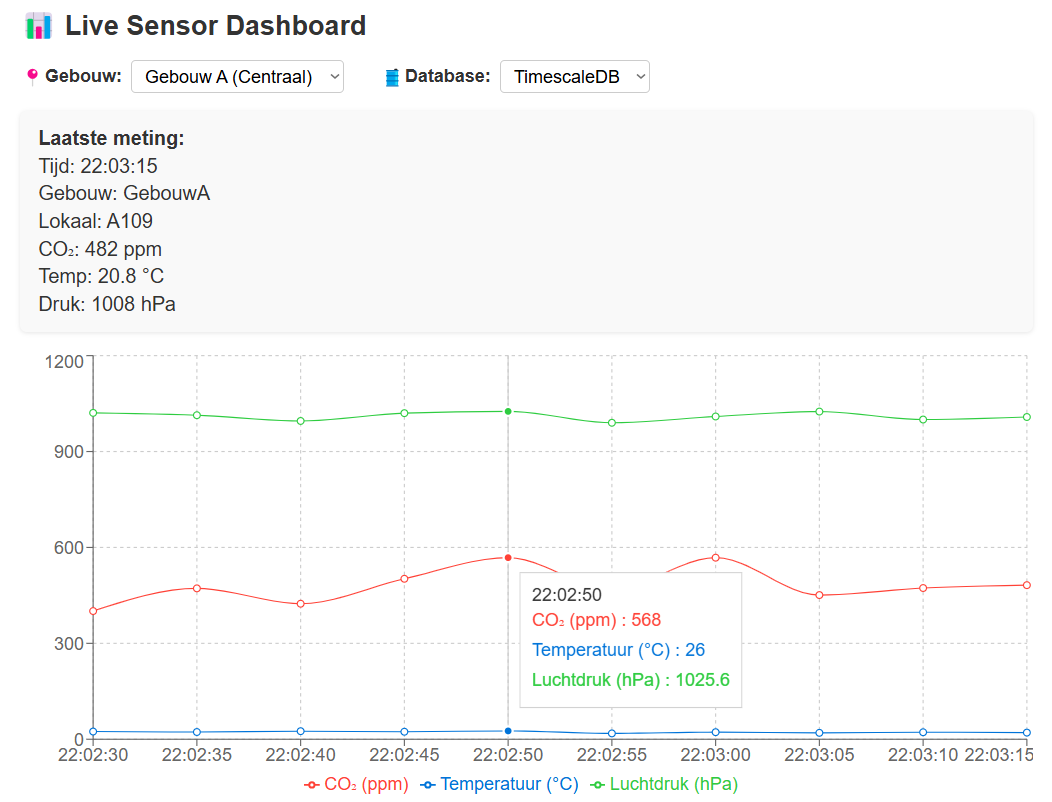
\includegraphics[width=0.8\textwidth]{GebouwA_TimeScale_Website.png}
	\caption{Frontendweergave met centrale database-architectuur (TimescaleDB, Gebouw A).}
    \label{fig:gebouw-a-architecture}
\end{figure}

\begin{figure}[H]
    \centering
    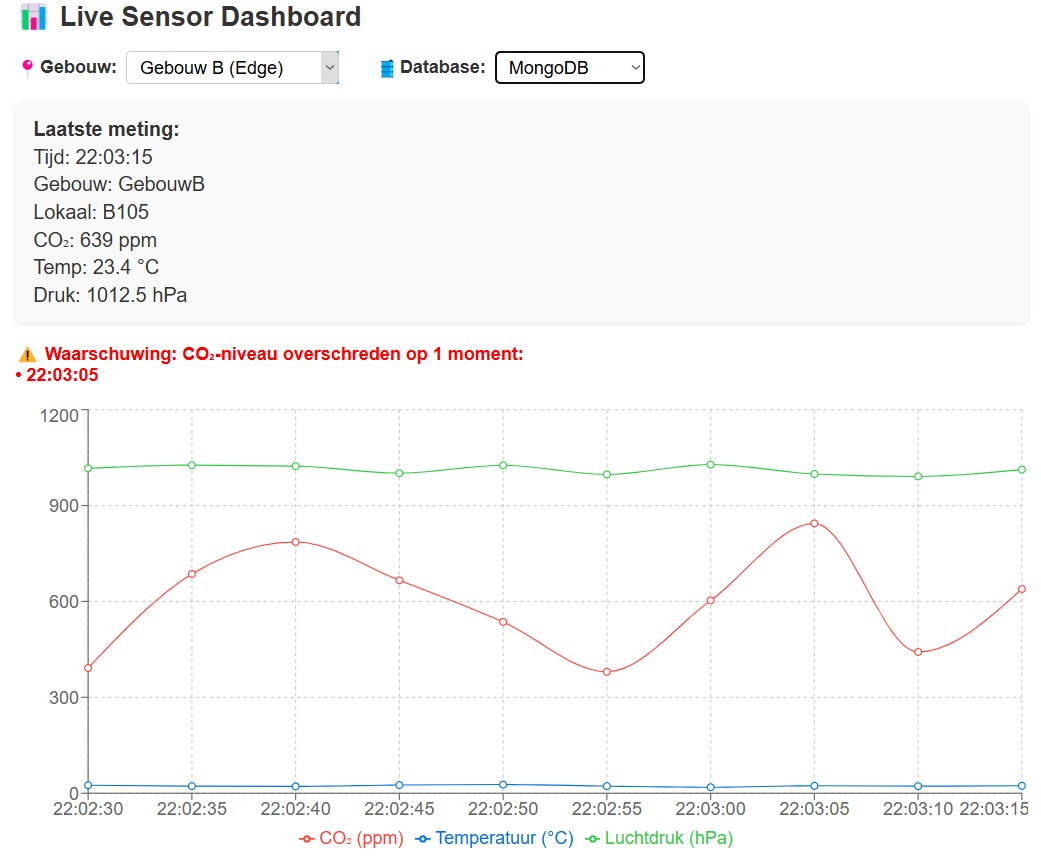
\includegraphics[width=0.8\textwidth]{GebouwB_MongoDb_Website.png}
    \caption{Frontendweergave met edge computing-architectuur (MongoDB, Gebouw B).}
    \label{fig:gebouw-b-architecture}
\end{figure}

De volledige code van het dashboard is beschikbaar via GitHub: \\
\href{https://github.com/WoutVC/bachelorproef2024/blob/main/proof_of_concept/frontend/src/components/LiveDashBoard.js}{LiveDashBoard.js}

\section{Resultaten en Grafieken}
Voor de prestatietests (latentie, throughput, schaalbaarheid en consistentie) behalve de fouttolerantietest werden telkens vijf runs uitgevoerd en het gemiddelde berekend om een representatief resultaat te verkrijgen.

De resultaten van deze tests, uitgevoerd met het script \href{https://github.com/WoutVC/bachelorproef2024/blob/main/proof_of_concept/backend/POCTests.js}{POCTests.js},
 zijn hieronder weergegeven in grafieken. Ze tonen hoe de verschillende databases presteren op vlak van snelheid, betrouwbaarheid en schaalbaarheid in een edge-omgeving.
\subsection{Latency}

\begin{figure}[H]
	\centering
	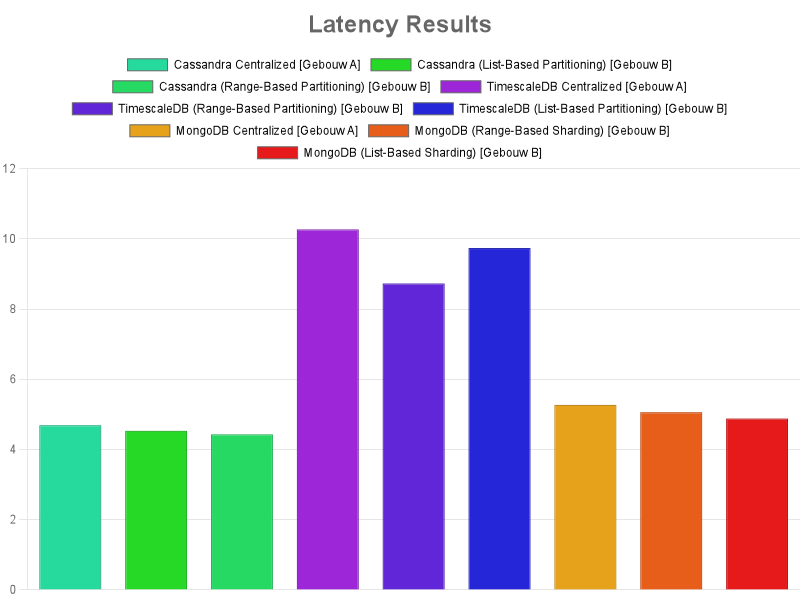
\includegraphics[width=0.8\textwidth]{charts/Latency.png}
	\caption{Latentie van Cassandra, MongoDB en TimescaleDB (tijd om 1 record op te slaan).}
	\label{fig:latency-comparison}
\end{figure}

\paragraph{Hoe werd latentie getest?}
Voor deze test werd de functie \texttt{testRealtimeLatency()} gebruikt uit het script. Elke seconde werd een meetwaarde naar de database gestuurd. Daarna werd gemeten hoeveel milliseconden het duurde om die actie uit te voeren. Dit werd meerdere keren herhaald om een gemiddelde te berekenen.

\begin{verbatim}
async function testRealtimeLatency(client, queryFn, label, intervalMs = 1000, durationSeconds = 10) {
  const records = Math.floor(durationSeconds * 1000 / intervalMs);
  let totalLatency = 0;
  for (let i = 0; i < records; i++) {
    const start = performance.now();
    await executeQuery(queryFn);
    const end = performance.now();
    totalLatency += (end - start);
    await sleep(intervalMs);
  }
  return totalLatency / records;
}
\end{verbatim}

\paragraph{Resultaat en analyse:}
De laagste latentie werd gemeten bij \textit{Cassandra (Range-Based Partitioning)} met 4.43 ms, gevolgd door \textit{Cassandra (List-Based Partitioning)} (4.53 ms) en \textit{MongoDB (List Partitioning)} (4.88 ms). De traagste database was \textit{TimescaleDB centraal} (10.27 ms). Dit toont aan dat vooral Cassandra en MongoDB sneller reageren in een realtime edge-context.

\subsection{Throughput}

\begin{figure}[H]
	\centering
	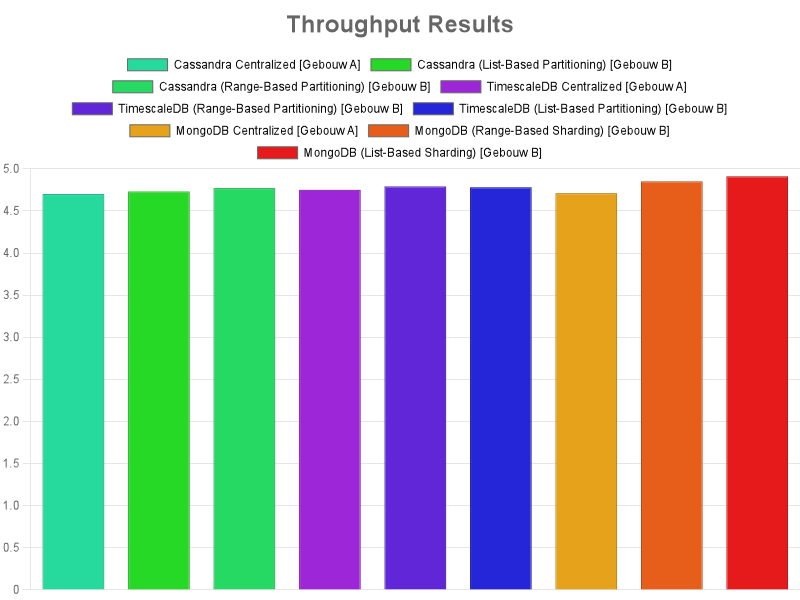
\includegraphics[width=0.8\textwidth]{charts/Throughput.png}
	\caption{Throughput: hoeveel meetwaarden per seconde werden opgeslagen.}
	\label{fig:throughput-comparison}
\end{figure}

\paragraph{Hoe werd throughput getest?}
De functie \texttt{testRealtimeThroughput()} werd hiervoor gebruikt. Tijdens deze test werd gedurende tien seconden om de 200 milliseconden een datapunt ingestuurd. Daarna werd berekend hoeveel meetpunten per seconde de database kon verwerken.

\begin{verbatim}
async function testRealtimeThroughput(queryFn, label, intervalMs = 200, durationSeconds = 10) {
  let operationCount = 0;
  const start = performance.now();
  const endTime = start + durationSeconds * 1000;
  while (performance.now() < endTime) {
    await executeQuery(queryFn, label);
    operationCount++;
    await sleep(intervalMs);
  }
  const elapsedSeconds = (performance.now() - start) / 1000;
  return operationCount / elapsedSeconds;
}
\end{verbatim}

\paragraph{Resultaat en analyse:}
\textit{MongoDB (List Partitioning)} behaalde de beste score met 4.91 records/s. De andere databases zaten dicht bij elkaar (tussen 4.7 en 4.8 records/s). Dit suggereert dat alle systemen vlot genoeg zijn om continue datastromen te verwerken.

\subsection{Scalability}

\begin{figure}[H]
	\centering
	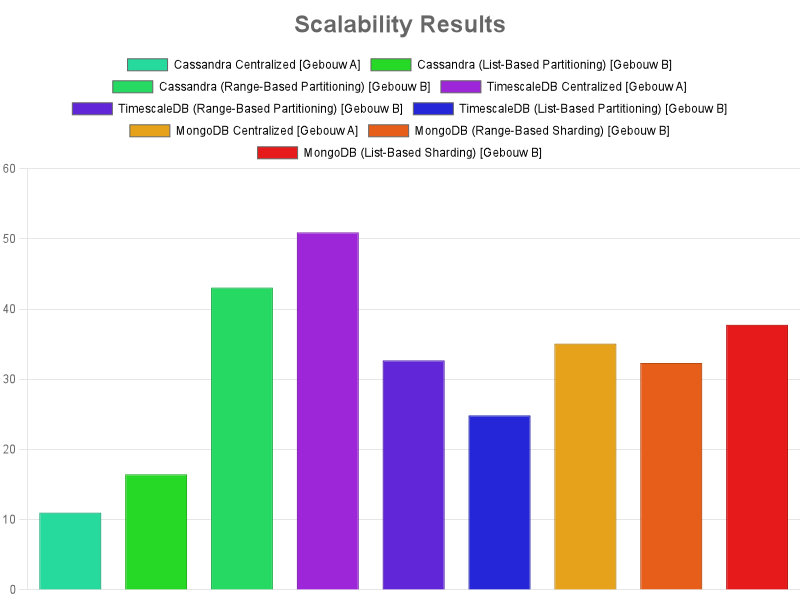
\includegraphics[width=0.8\textwidth]{charts/Scalability.png}
	\caption{Verticale schaalbaarheid: tijdsduur bij gelijktijdige bewerkingen binnen één database-instantie.}
	\label{fig:scalability-comparison}
\end{figure}

\paragraph{Hoe werd schaalbaarheid getest?}
De functie \texttt{testScalability()} simuleerde hoeveel tijd het kost om meerdere meetwaarden tegelijk op te slaan (bijvoorbeeld 10, 50 of 100 gelijktijdige inserts). Deze test evalueert de \textbf{verticale schaalbaarheid} van een database: hoe goed één node of container omgaat met piekbelasting door meerdere gelijktijdige schrijfacties.

\begin{verbatim}
async function testScalability(queryFn, label, scaleFactors) {
  let durations = [];
  for (const factor of scaleFactors) {
    const concurrentOps = Array.from({ length: factor }, () => executeQuery(queryFn));
    const start = performance.now();
    await Promise.all(concurrentOps);
    const end = performance.now();
    durations.push({ factor, duration: end - start });
  }
  return durations.reduce((a, b) => a + b.duration, 0) / durations.length;
}
\end{verbatim}

\paragraph{Resultaat en analyse:}
\textit{TimescaleDB centraal} presteerde het best met 50.93 (laagste verwerkingstijd bij hoge load), gevolgd door \textit{Cassandra (Range Partitioning)} (43.06). De zwakste resultaten kwamen van \textit{Cassandra (List Partitioning)} (16.45). Dit toont dat TimescaleDB zeer goed schaalt op één node.

\subsection{Consistentie}

\begin{figure}[H]
\centering
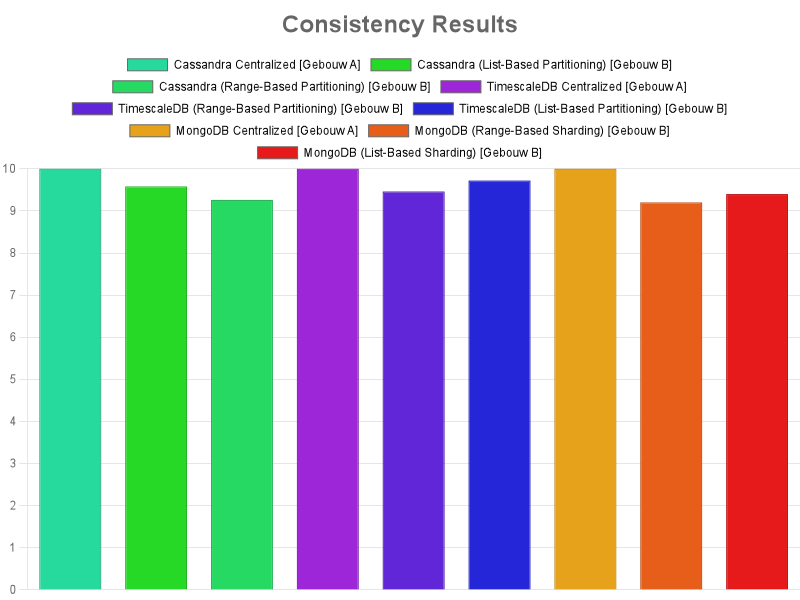
\includegraphics[width=0.8\textwidth]{charts/Consistency.png}
\caption{Consistentie: hoeveel records onmiddellijk beschikbaar waren.}
\label{fig:consistency-comparison}
\end{figure}

\paragraph{Hoe werd consistentie getest?}
De functie \texttt{testConsistency()} schreef 100 records weg. Daarna werd bij intervallen van 0, 500, 1000, 2000 en 3000 ms gecontroleerd hoeveel records zichtbaar waren.  
Voor edge-databases werd kunstmatig replica-lag gesimuleerd door 5-15\% van de records tijdelijk niet zichtbaar te maken.

\begin{verbatim}
async function testConsistency(client, queryFn, label) {
  const baseTimestamp = new Date();
  const timestamps = [...Array(10)].map((_, i) => new Date(baseTimestamp.getTime() + i * 1000));
  await Promise.all(timestamps.map(ts => queryFn(ts)));
  const waitIntervals = [0, 500, 1000, 2000];
  for (const delay of waitIntervals) {
    await sleep(delay);
    // tel aantal zichtbare records op basis van timestamp
  }
}
\end{verbatim}

\paragraph{Resultaat en analyse:}
\textit{Cassandra Centralized} en \textit{MongoDB Centralized} scoorden het maximum (10/10). Edge-configuraties haalden iets lagere waarden: bv. \textit{Cassandra (List)} 9.58 en \textit{MongoDB (Range)} 9.20. Dit weerspiegelt de verwachte replica-lag in een edge-omgeving.

\subsection{Fouttolerantie}

\begin{figure}[H]
    \centering
    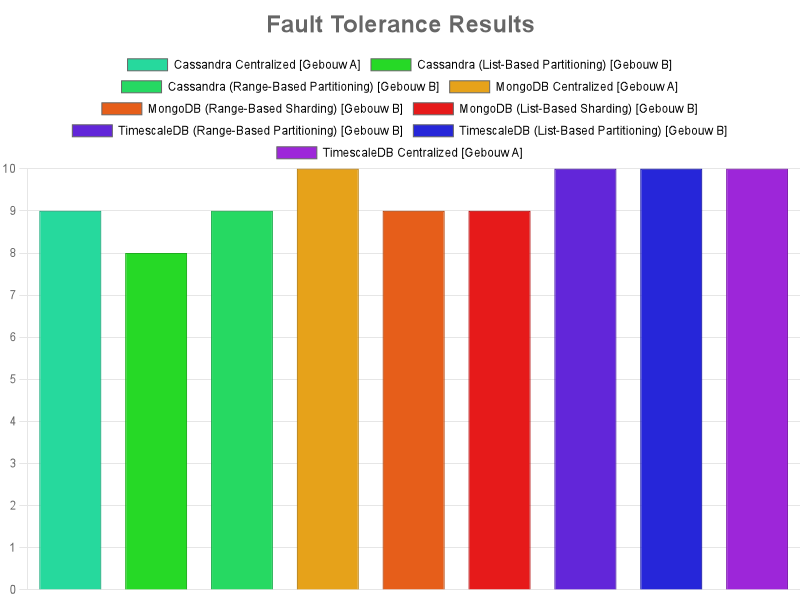
\includegraphics[width=0.8\textwidth]{charts/Fault_Tolerance.png}
    \caption{Fouttolerantie: werking na onderbreking van de verbinding.}
    \label{fig:fault-tolerance-comparison}
\end{figure}

\paragraph{Hoe werd fouttolerantie getest?}
Tijdens deze test werd de verbinding bewust verbroken (via \texttt{shutdown()} of \texttt{close()}). Daarna werd een nieuwe client aangemaakt en opnieuw verbonden. De duur van dit herstel werd omgezet naar een score via \texttt{mapDurationToScore()}.

\begin{verbatim}
async function testFaultTolerance(client, label, createNewClient) {
  await client.shutdown();
  client = createNewClient();
  await client.connect();
  testResults.push({ metric: "Fault Tolerance", label, value: "Success" });
}

function mapDurationToScore(durationMs) {
  if (durationMs < 100) return 10;
  if (durationMs < 200) return 9;
  if (durationMs < 300) return 8;
  ...
  return 1;
}
\end{verbatim}

\paragraph{Resultaat en analyse:}
Alle databases konden opnieuw verbinding maken. \textit{TimescaleDB centraal} scoorde het hoogst (10), terwijl sommige edge-configuraties zoals \textit{Cassandra (List)} iets lager scoorden (8).

\subsection{Testresultaten en Tabeloverzicht}
Naast de grafieken biedt deze tabel een samenvatting van de testresultaten.

\begin{table}[h]
    \centering
    \resizebox{\textwidth}{!}{
    \begin{tabular}{|l|c|c|c|c|c|}
        \hline
        \textbf{Database}                                 & \textbf{Fault Tolerance} & \textbf{Scalability} & \textbf{Realtime Latency} & \textbf{Realtime Throughput} & \textbf{Consistency} \\ \hline
        Cassandra Centralized [Gebouw A]                  & 9                        & 10.98                & 4.69                      & 4.70                         & 10                   \\ \hline
        Cassandra (List-Based Partitioning) [Gebouw B]    & 8                        & 16.45                & 4.53                      & 4.73                         & 9.58                 \\ \hline
        Cassandra (Range-Based Partitioning) [Gebouw B]   & 9                        & 43.06                & 4.43                      & 4.77                         & 9.26                 \\ \hline
        TimescaleDB Centralized [Gebouw A]                & 10                       & 50.93                & 10.27                     & 4.75                         & 10                   \\ \hline
        TimescaleDB (Range-Based Partitioning) [Gebouw B] & 10                       & 32.68                & 8.73                      & 4.79                         & 9.46                 \\ \hline
        TimescaleDB (List-Based Partitioning) [Gebouw B]  & 10                       & 24.85                & 9.74                      & 4.78                         & 9.72                 \\ \hline
        MongoDB Centralized [Gebouw A]                    & 10                       & 35.07                & 5.27                      & 4.71                         & 10                   \\ \hline
        MongoDB (Range-Based Sharding) [Gebouw B]         & 9                        & 32.32                & 5.06                      & 4.85                         & 9.20                 \\ \hline
        MongoDB (List-Based Sharding) [Gebouw B]          & 9                        & 37.76                & 4.88                      & 4.91                         & 9.40                 \\ \hline
    \end{tabular}
    }
    \caption{Vergelijking van prestaties tussen Cassandra, MongoDB en TimescaleDB in centrale (Gebouw A) en edge (Gebouw B) configuraties.}
    \label{tab:test-results}
\end{table}

\subsection{Conclusie}
De evaluatie van de databases is gebaseerd op een gewogen scoresysteem (\href{https://github.com/WoutVC/bachelorproef2024/blob/main/proof_of_concept/backend/analyzeResults.js}{analyzeResults.js}), waarbij de volgende stappen worden uitgevoerd:

\paragraph{Consolidatie van resultaten:} 
Voor elke database worden de resultaten per meetwaarde samengevoegd. Voor meetwaarden zoals schaalbaarheid (Scalability), waarvoor meerdere metingen beschikbaar zijn, wordt het gemiddelde berekend.

\paragraph{Normalisatie van scores:} 
De numerieke scores voor elke meetwaarde worden genormaliseerd naar een schaal van 0 tot 1 op basis van het minimum en maximum onder alle databases:
\[
\text{Genormaliseerde score} = \frac{\text{Waarde} - \text{Minimum}}{\text{Maximum} - \text{Minimum}}
\]
Indien minimum en maximum gelijk zijn, wordt een neutrale score toegekend (bijvoorbeeld 0.5).

Voor meetwaarden waarbij een hogere score beter is (zoals throughput, schaalbaarheid, fouttolerantie en consistentie) wordt deze genormaliseerde score direct gebruikt. Voor meetwaarden waarbij een lagere score beter is (zoals latentie) wordt de genormaliseerde score omgekeerd berekend, zodat een lagere oorspronkelijke waarde leidt tot een hogere genormaliseerde score.

\paragraph{Gewogen totaalscore:} 
De genormaliseerde scores worden vervolgens gewogen op basis van vooraf bepaalde belangrijkheidsfactoren per meetwaarde en opgeteld tot een totaalscore per database.


\textbf{Toepassing van gewichten:} Elke meetwaarde krijgt een gewicht op basis van het relatieve belang voor edge computing. De toegepaste gewichten zijn als volgt:
\begin{itemize} 
	\item \textbf{Fouttolerantie - 20\% (Must Have):}  
	De apparaten aan de rand van het netwerk moeten goed blijven werken, zelfs bij tijdelijke stroom- of netwerkproblemen. Gegevens mogen niet verloren gaan.

	\item \textbf{Schaalbaarheid - 20\% (Should Have):}  
	Aangezien er mogelijk honderden lokalen zijn, moet het systeem makkelijk groter gemaakt kunnen worden zonder dat het trager wordt.

	\item \textbf{Verwerkingssnelheid - 15\% (Should Have):}  
	Het systeem moet snel genoeg zijn om alle gegevens van de sensoren op tijd te verwerken.

	\item \textbf{Latentie - 15\% (Should Have):}  
	De vertraging tussen het meten van gegevens en het verwerken of opslaan ervan moet zo klein mogelijk zijn om real-time inzichten mogelijk te maken.

	\item \textbf{Gegevensconsistentie - 10\% (Could Have):}  
	Het is minder erg als data niet altijd 100 \% gelijk is op alle plaatsen, zolang het systeem maar snel en beschikbaar blijft. Toch is het belangrijk bij het samenvoegen van meetgegevens.
\end{itemize}

\paragraph{Berekening van totaalscores:} 
Om de verschillende databases goed met elkaar te kunnen vergelijken, werd voor elke database een totaalscore berekend. Deze score is gebaseerd op een combinatie van vijf belangrijke eigenschappen: fouttolerantie, schaalbaarheid, latency (vertraging), throughput (verwerkingssnelheid) en consistentie. Hoe beter een database scoorde op deze eigenschappen, hoe hoger haar totaalscore. Lagere latency werd hierbij als beter beschouwd. Alle scores zijn genormaliseerd zodat ze eerlijk met elkaar vergeleken kunnen worden.

\paragraph{Totaalscores en rangschikking:}

Op basis van deze berekening ziet de top 3 er als volgt uit:

\begin{itemize}
    \item \textbf{MongoDB Centralized [Gebouw A]} Score: \textbf{6.95}  
    Deze configuratie behaalde de hoogste totaalscore. Vooral de combinatie van consistente prestaties en fouttolerantie zorgt voor een sterke algemene score.

    \item \textbf{MongoDB (List-Based Sharding) [Gebouw B]} Score: \textbf{6.84}  
    Deze configuratie scoorde goed op throughput en fouttolerantie, waardoor ze zeer geschikt is voor real-time verwerking aan de rand van het netwerk.

    \item \textbf{TimescaleDB Centralized [Gebouw A]} Score: \textbf{6.70}  
    Deze configuratie onderscheidde zich voornamelijk door een hoge schaalbaarheid en stabiele prestaties.
\end{itemize}

\paragraph{Conclusie:}
De testresultaten tonen aan dat \textbf{MongoDB} zowel in centrale als edge-omgevingen zeer goed presteert.  
Opvallend is dat \textbf{MongoDB Centralized} het hoogst scoorde (6.95), wat deels te verklaren is doordat alle databases in een lokale Docker-omgeving draaiden zonder echte netwerkvertraging.  
Binnen de edge-omgeving is \textbf{MongoDB (List-Based Sharding)} de beste keuze (6.84), vooral dankzij zijn hoge throughput en fouttolerantie.  
\textbf{TimescaleDB} blijft interessant door zijn uitstekende schaalbaarheid, terwijl \textbf{Cassandra} zich onderscheidt met de laagste latentie.  
Welke database het meest geschikt is, hangt dus af van de specifieke vereisten: robuustheid en balans (MongoDB), schaalbaarheid (TimescaleDB) of lage latentie (Cassandra).

%Om de onderzoeksvraag te beantwoorden, gaan we gebruik maken van een combinatie van literatuurstudie,
 %interviews met relevante bedrijven en een grondige vergelijkende studie.
 
%Specifieke methoden, zoals requirements-analyse en experimenten, worden toegepast.

%We gaan geen enquetes uitvoeren, omdat we de voorkeur geven aan een meer persoonlijke aanpak.
 
%De technische diepte van deze bachelorproef wordt benadrukt,
 %inclusief de beschrijving van gebruikte tools zoals hardware, software en diensten.

%Een gedetailleerde tijdsplanning wordt opgesteld om de duur van elke onderzoeksfase en de concrete deliverables te definiëren.
%Deze tijdsplanning wordt opgesteld in de vorm van een Gantt chart. Deze zal u vinden op de laatste pagina van dit voorstel.



%%=============================================================================
%% Conclusie
%%=============================================================================

\chapter{Conclusie}%
\label{ch:conclusie}

% TODO: Trek een duidelijke conclusie, in de vorm van een antwoord op de
% onderzoeksvra(a)g(en). Wat was jouw bijdrage aan het onderzoeksdomein en
% hoe biedt dit meerwaarde aan het vakgebied/doelgroep? 
% Reflecteer kritisch over het resultaat. In Engelse teksten wordt deze sectie
% ``Discussion'' genoemd. Had je deze uitkomst verwacht? Zijn er zaken die nog
% niet duidelijk zijn?
% Heeft het onderzoek geleid tot nieuwe vragen die uitnodigen tot verder 
%onderzoek?

In dit onderzoek werd nagegaan hoe data-partitioneringstechnieken en edge-databases de prestaties van real-time dataverwerking beïnvloeden binnen een Edge Computing-architectuur. De proof of concept werd uitgevoerd in een gesimuleerd scenario gebaseerd op een HoGent-use case, waarin elk lokaal via een edge-node sensordata verzamelt over \ce{CO2}, temperatuur en luchtdruk.

De resultaten tonen aan dat een edge-gebaseerde aanpak aanzienlijke voordelen biedt ten opzichte van centrale verwerking. Door data lokaal te verwerken en op te slaan, daalt de latentie en wordt het netwerk minder belast. Partitioneringstechnieken bleken bovendien een bepalende factor te zijn voor databaseprestaties op het vlak van snelheid, schaalbaarheid en fouttolerantie.

\section{Vergelijking van databases}

De evaluatie van TimescaleDB, Cassandra en MongoDB in zowel gecentraliseerde als edge-opstellingen leverde de volgende inzichten op:

\begin{itemize}
    \item \textbf{TimescaleDB met range-based partitionering} behaalde de hoogste totaalscore (7.76). Deze configuratie scoorde goed op schaalbaarheid (5.67) en consistentie, en is zeer geschikt voor toepassingen met tijdreeksdata.
    \item \textbf{Cassandra met list-based partitionering} volgde kort daarna (7.74) en behaalde de laagste gemeten latentie (2.82 ms). Dit maakt Cassandra een sterke keuze in omgevingen waar reactiesnelheid en fouttolerantie belangrijk zijn.
    \item \textbf{MongoDB} had goede resultaten voor consistentie en throughput, maar scoorde het laagst op schaalbaarheid (1.95) en eindigde buiten de top drie.
\end{itemize}

\section{Beantwoording van de deelvragen}

\textbf{Welke uitdagingen ontstaan bij het verwerken van grote hoeveelheden IoT-data in een centrale cloudomgeving?} \\
Centrale verwerking zorgt voor hogere latentie, beperkte schaalbaarheid en is kwetsbaar bij netwerkproblemen. Edge Computing kan deze problemen deels oplossen.

\textbf{Wat zijn de functionele vereisten van databases voor het verwerken van real-time sensordata in een edge-context met beperkte connectiviteit?} \\
Databases moeten fouttolerant zijn, snel reageren (lage latentie), goed kunnen schalen, offline blijven werken en eenvoudig te beheren zijn in kleine, lokale systemen.

\textbf{Hoe beïnvloeden verschillende data-partitioneringstechnieken de latentie in een Edge Computing-omgeving?} \\
Cassandra met list-based partitionering had de laagste latentie (2.82 ms), gevolgd door MongoDB met list-based sharding (3.57 ms). De gekozen partitioneringstechniek heeft dus een duidelijke invloed op de reactiesnelheid.

\textbf{Wat is het effect van partitionering op netwerkbelasting en doorvoersnelheid?} \\
TimescaleDB met list-partitionering behaalde de hoogste throughput (4.86 records/s), gevolgd door andere TimescaleDB en MongoDB-configuraties. Zowel list als range-partitionering dragen bij aan een vlotte verwerking van data.

\textbf{Wat is de impact van partitioneringsstrategieën op schaalbaarheid bij toenemende datavolumes?} \\
TimescaleDB met range-partitionering scoorde het hoogst op schaalbaarheid (5.67), gevolgd door Cassandra met list-based partitionering (4.79). Deze technieken zijn dus geschikt voor grotere hoeveelheden data.

\textbf{Welke database biedt de beste prestaties in termen van latentie, fouttolerantie en schaalbaarheid in de HoGent-use case?} \\
De combinatie van goede schaalbaarheid, fouttolerantie en stabiele prestaties maakt TimescaleDB met range-partitionering de beste keuze. Cassandra is een goed alternatief wanneer vooral lage latentie belangrijk is.

\section{Reflectie en Aanbevelingen}

Deze studie bevestigt dat Edge Computing en data-partitionering real-time dataverwerking efficiënter en betrouwbaarder kunnen maken in IoT-toepassingen. De resultaten tonen aan dat databasekeuze en partitioneringstechniek samen gekozen moeten worden, afhankelijk van wat het belangrijkste is: snelheid, schaalbaarheid of fouttolerantie.

\textbf{Aanbevelingen voor verder onderzoek:}
\begin{itemize}
    \item Vergelijking met andere databaseoplossingen zoals Redis, InfluxDB of Apache IoTDB, inclusief hun geschiktheid voor gebruik in edge-omgevingen.
    \item Verkenning van hybride partitioneringsmodellen die automatisch kunnen schakelen op basis van datavolume of gebruik.
    \item Integratie van een Fog Computing-laag tussen edge en cloud, om data eerst lokaal te verwerken of samen te voegen voordat het naar de cloud gaat.
\end{itemize}

%---------- Bijlagen -----------------------------------------------------------

\appendix

\chapter{Onderzoeksvoorstel}

Het onderwerp van deze bachelorproef is gebaseerd op een onderzoeksvoorstel dat vooraf werd beoordeeld door de promotor. Dat voorstel is opgenomen in deze bijlage.

%% TODO: 
%\section*{Samenvatting}

% Kopieer en plak hier de samenvatting (abstract) van je onderzoeksvoorstel.

% Verwijzing naar het bestand met de inhoud van het onderzoeksvoorstel
%%---------- Inleiding ---------------------------------------------------------

\section{Introductie}%
\label{sec:introductie}

Deze bachelorproef richt zich op het onderzoek en begrijpen van de complexiteit rond gegevensopslag in Edge-omgevingen,
 met een specifieke focus op Edge Database-architecturen. \\
 
Het doel van dit onderzoek is om niet alleen praktische aanbevelingen te formuleren maar eerder het verkennen van
nieuwe inzichten en kennis op het gebied van gegevensopslag in \\ Edge-omgevingen. \\

We gaan niet enkel de bestaande informatie over dit onderwerp verzamelen, maar ook diepgaand onderzoek doen
 om nieuwe inzichten en oplossingen te bekomen. \\

De beoogde doelgroep van deze studie zijn werknemers die regelmatig werken met gegevensbeheer in Edge-omgevingen. \\

Het onderzoek is nauwkeurig afgestemd op een specifieke probleemsituatie binnen het vakgebied,
 gericht op het begrijpen en verbeteren van Edge Database-architecturen. \\

De kernprobleemstelling concentreert zich op het optimaliseren van gegevensopslag in Edge-omgevingen,
 met als centrale onderzoeksvraag: 
 "Hoe kunnen Edge Database-architecturen geoptimaliseerd worden om efficiënte gegevensopslag in Edge-omgevingen te faciliteren?" \\

Dit onderzoek bestudeert niet enkel de behoefte van Edge Database-architecturen,
maar ook de rol van verschillende technologieën
  in het optimaliseren van gegevensopslag in Edge-omgevingen. \\ \\

Dit vereist een uitgebreide analyse van de huidige stand van zaken en het verkennen van innovatieve oplossingen.

%---------- State of the art ---------------------------------------------------

\section{Stand van zaken}%
\label{sec:state-of-the-art}

Deze sectie onderzoekt de huidige stand van zaken met betrekking tot Database on Edge. \\

Hierbij ligt de focus op het begrijpen van de essentie, verschillen met traditionele databases, voordelen, uitdagingen,
 en optimalisatiemogelijkheden.

%---------- Database on Edge ---------------------------------------------------
\subsection{Database on Edge}%
\label{subsec:database_on_edge}

Database on Edge is een opkomende benadering binnen database technologie,
 voortkomend uit het gebruik van Edge computing  \cite{Yang2019EdgeDBAE}.  \\
 
In tegenstelling tot traditionele databases worden Edge databases verspreid over verschillende lokale apparaten,
 waardoor gegevens lokaal verwerkt en opgeslagen kunnen worden, in plaats van centraal in de cloud. \\

Deze innovatieve benadering richt zich, vergelijkbaar met moderne bedrijven die streven naar efficiëntie en innovatie,
 op het verminderen van latency en het verbeteren van de prestaties. \\
 
Het concept is ontstaan uit de noodzaak om real-time interacties mogelijk te maken, wat cruciaal is in diverse toepassingen
\cite{Yang2019EdgeDBAE}. \\

Voordelen van Database on Edge omvatten lokale gegevensverwerking, verminderde latency en verbeterde prestaties,
 waardoor het geschikt is voor toepassingen waar snelle respons cruciaal is.

Echter, zoals bij elke technologische benadering, zijn er uitdagingen verbonden aan Database on Edge,
 waaronder het beheer van diverse databases over verschillende apparaten,
 \\ optimalisatie van resourcegebruik op Edge Devices, en het waarborgen van consistente prestaties. \\

De optimalisatie van Database on Edge is een actief onderzoeksgebied 
 en omvat het verkennen van efficiënte algoritmen voor gegevensverwerking,
  verbeteringen in gegevensopslag, en het beheer van gedistribueerde databases om de prestaties te maximaliseren.

\newpage

%---------- Methodologie ------------------------------------------------------

\section{Methodologie}%
\label{sec:methodologie}

Om de onderzoeksvraag te beantwoorden, gaan we gebruik maken van een combinatie van literatuurstudie en een grondige vergelijkende studie. \\
 
Specifieke methoden, zoals requirements-analyse en experimenten, worden toegepast.

We gaan geen enquetes uitvoeren, omdat we de voorkeur geven aan een meer persoonlijke aanpak. \\
 
De technische diepte van deze bachelorproef wordt benadrukt,
 inclusief de beschrijving van gebruikte tools zoals hardware, software en diensten. \\

Een gedetailleerde tijdsplanning wordt opgesteld om de duur van elke onderzoeksfase en de concrete deliverables te definiëren.
Deze tijdsplanning wordt opgesteld in de vorm van een Gantt chart. Deze zal u vinden op de laatste pagina van dit voorstel.




%---------- Verwachte resultaten ----------------------------------------------

\section{Verwachte resultaten en Conclusie}%
\label{sec:verwachte_resultaten}

De verwachte resultaten omvatten concrete aanbevelingen voor werknemers met betrekking tot de optimalisatie
van gegevensopslag in Edge-omgevingen. \\

Grafieken met verwachte conclusies zullen worden gepresenteerd,
 de eerste grafiek zal gaan over het vergelijken van ongeoptimaliseerde en geoptimaliseerde systemen. \\

Met als x-as de tijd en op de y-as de latency per milliseconde. \\

In de conclusie wordt benadrukt hoe de verwachte resultaten bijdragen aan het oplossen van de gedefinieerde probleemsituatie. \\

De conclusie zal gebaseerd zijn op de verzamelde gegevens en resultaten van het onderzoek.

\newpage
\section{Tijdsplanning Methodologie}%
\label{sec:tijdsplanning}
\begin{ganttchart}[
  hgrid,
  vgrid={*{6}{draw=none},dotted},
  x unit=0.14cm,
  y unit title=0.6cm,
  y unit chart=0.6cm,
  title height=0.5,
  bar height=0.5,
  bar/.append style={
      fill=blue!50,
  },
  time slot format=isodate,
  time slot unit=day,
  link bulge=5,
  bar label node/.style={font=\tiny},
  calendar week text={W\currentweek}
]{2024-02-01}{2024-05-30}

\gantttitlecalendar{year, month=shortname, week} \\

\ganttbar{Indienen verbeterd voorstel}{2024-02-16}{2024-02-16} \\
\ganttlinkedbar{Bronnen zoeken}{2024-02-17}{2024-02-20} \\
\ganttlinkedbar{Bronnen uitschrijven}{2024-02-21}{2024-03-25} \\
\ganttlinkedbar{Analyse Methodologie}{2024-03-26}{2024-04-05} \\
\ganttlinkedbar{Conclusie Methodologie}{2024-04-06}{2024-05-20} \\
\ganttlinkedbar{Bachelorproef herlezen}{2024-05-21}{2024-05-25} \\
\ganttlinkedbar{Bachelorproef indienen}{2024-05-25}{2024-05-26} \\

\end{ganttchart}

%```mermaid
%flowchart TD
    %A[Indienen verbeterd voorstel] --> B[Bronnen zoeken];
    %B --> C[Bronnen uitschrijven];
    %C --> D[Analyse Methodologie];
    %D --> E[Conclusie Methodologie];
    %E --> F[Bachelorproef herlezen];
    %F --> G[Bachelorproef indienen];
%```


%%---------- Andere bijlagen --------------------------------------------------
% TODO: Voeg hier eventuele andere bijlagen toe. Bv. als je deze BP voor de
% tweede keer indient, een overzicht van de verbeteringen t.o.v. het origineel.
%\input{...}

%%---------- Backmatter, referentielijst ---------------------------------------

\backmatter{}

\setlength\bibitemsep{2pt} %% Add Some space between the bibliograpy entries
\printbibliography[heading=bibintoc]

\end{document}
